\chapter{Mérési eredmények}
%%%%%%%%%%%%%%%%%%%%%%%%%%%%%%%%%%%%%%%%%%%%%%%%%
%(12-15 oldal)



%\section{Mérési eredmények}
%(7-10 oldal): kinyert mérések tartalma(delay, jitter, link, AS info, Geolocation), mérések mennyisége, mérések minősége

\section{Létrehozott adatbázis bemutatása}
Jelen fejezet bemutatja a létrehozott adatbázis fontosabb adathalmazait, amelyek további elemzések alapját képezi.

\subsection*{Éllista}
A legfontosabb eredmény az internetes útvonalakat alkotó gépek közötti kapcsolatokról szolgáltat mérési eredményeket. Az objektum amelyről a mérés készült egy internetes link, a kinyert információk a következők:

\begin{itemize}
\item \textbf{delay:} késleltetés a két gép közötti kapcsolaton
\item \textbf{rtt:} A from számítógéphez végzett körülfordulási idő a mérést végző measurer\_ip számítógéptől
\item \textbf{time:} A mérés időpontja
\item \textbf{jitter:} Késleltetés ingadozás a két számítógép között
\item \textbf{measurer\_ip:} A mérést végző számítógép (ahol a traceroute parancs fut)
\item \textbf{target\_ip:} Az útvonalmérés célpontja
\item \textbf{to:} A mérést végző számítógéptől távolabbi csomópont információi: city, country, longitude, latitude, ip, asn
\item \textbf{from:} A mérést végző számítógéphez közelebbi csomópont információi: city, country, longitude, latitude, ip, asn
\end{itemize}

\subsection*{PlanetLab gépek állapota}
A PlanetLab gépek eléréséről (az operációs rendszeréről) és hiba esetén a hibaüzenetek aggregált statisztikája. A következő adatokat tartalmazza:

\begin{itemize}
\item \textbf{erroneous:} Sikertelen csatlakozások száma (online gépek esetén)
\item \textbf{succeed:} Gépek száma, amelyeken sikeres volt a távoli parancsfuttatás (cat /etc/issue)
\item \textbf{online:} A ping parancssal elérhető gépek száma
\item \textbf{offline:} A ping parancssal nem elérhető gépek száma
\item \textbf{outputs:} Az összes különböző kimenet felsorolása a hozzá tartozó előfordulások számával.
\item \textbf{error\_types:} Az összes különböző hibatípus felsorolása a hozzá tartozó előfordulások számával
\item \textbf{ts:} A mérés időpontja
\end{itemize}

\subsection*{AS gráf él információi}
A korábban részletesen bemutatott AS gráf ezen kollekció adataiból lett felépítve:

\begin{itemize}
\item \textbf{asn:} A autonóm rendszer azonosító száma
\item \textbf{core\_ips:} Az autonóm rendszeren belül észlelt ip címek
\item \textbf{gateways\_to\_as:} Az autonóm rendszerből másikba vezető kapcsolatok listája. A másik AS-hez irányuló ip cím párok (egyik AS kimeneti címe, másik AS bemeneti címe) listáit is tartalmazza.
\end{itemize}


\section{Gráf ábrázolása}

Az gráf tulajdonságainak intuitív leolvasásához ábrázolások készültek. Mivel már egy mérés során több mint 1700 csomópontból álló gráfot kell ábrázolni, ezért ennek kivitelesése nehézségekbe ütközik. A \ref{fig:graph} ábrán látható egy ilyen gráf leképezés.

\begin{figure}[!ht]
	\centering
	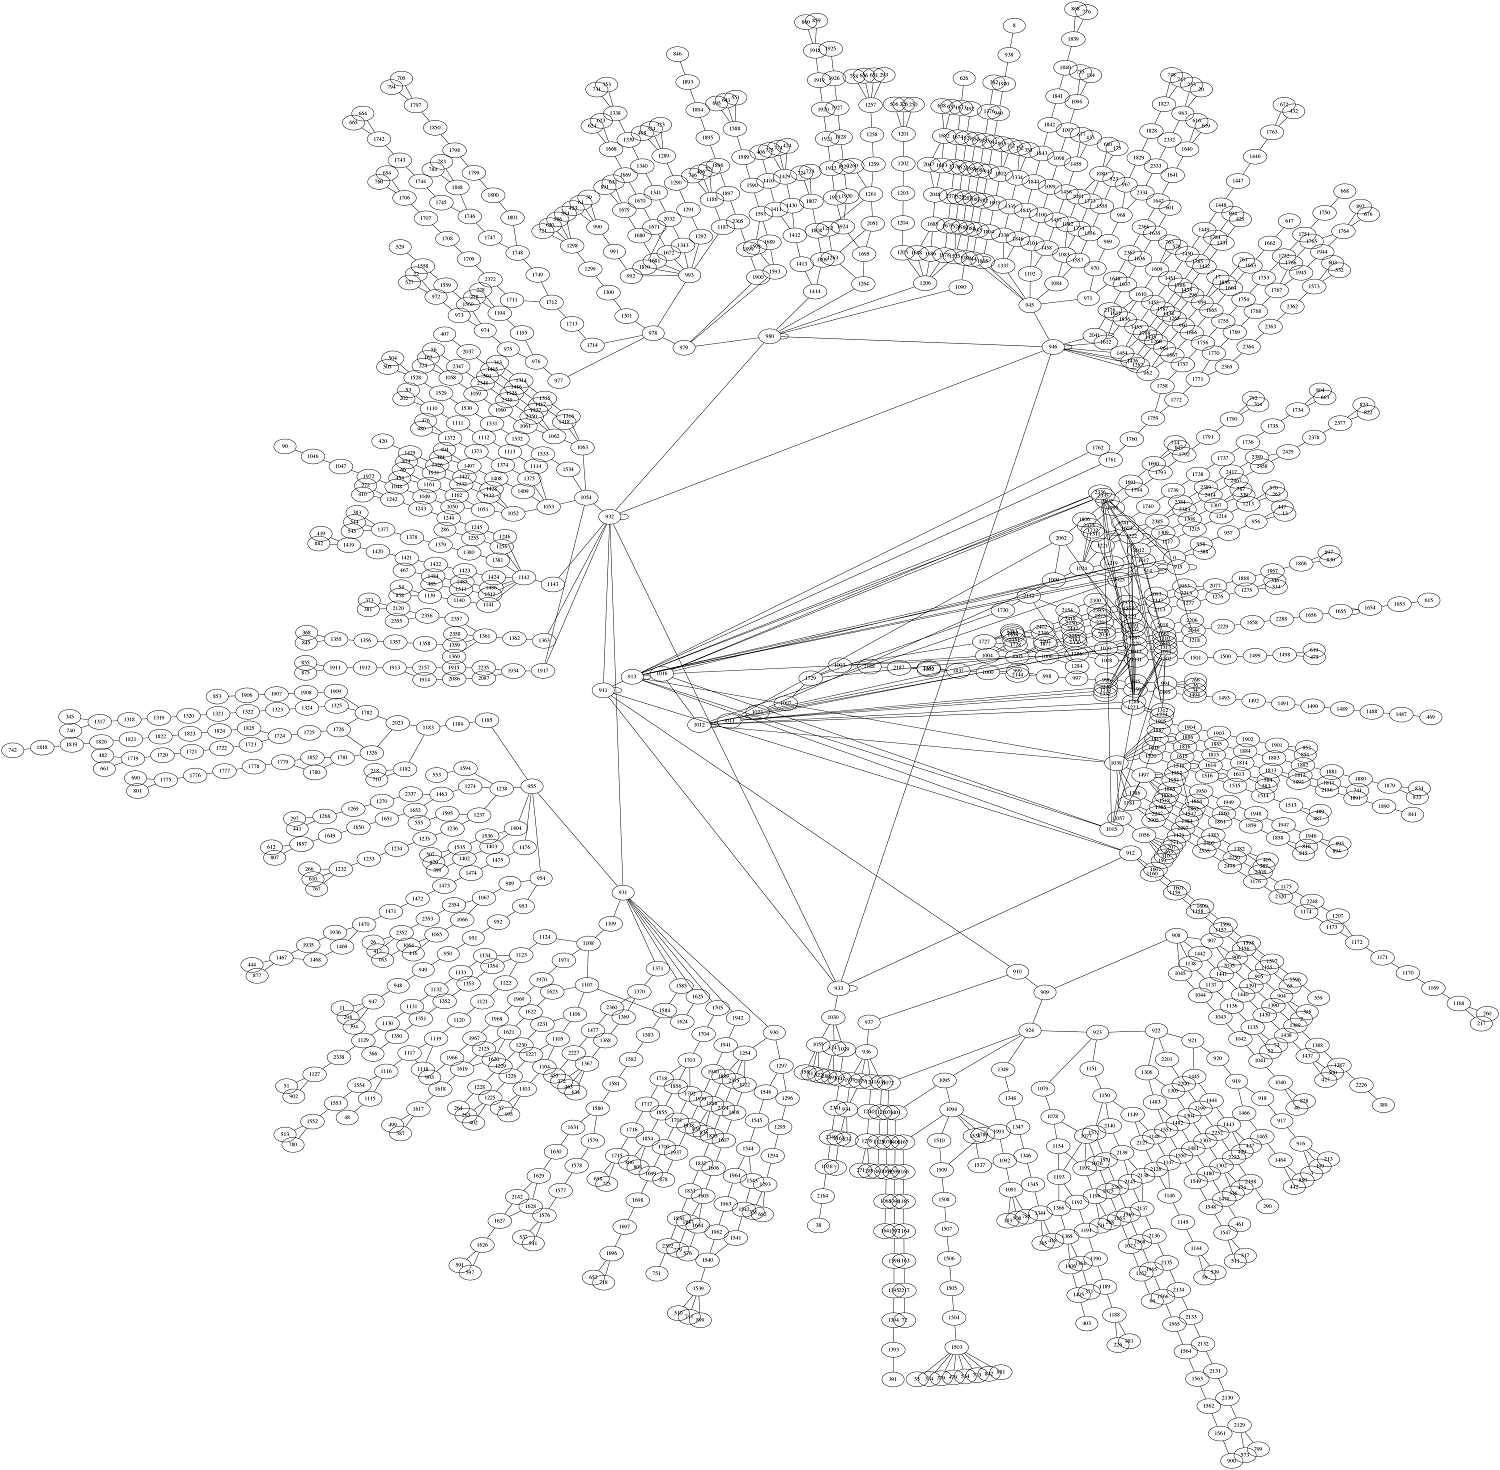
\includegraphics[width=1\textwidth, keepaspectratio]{figures/graph.png}
	\caption{Egy napi mérés gráfja csak az egyik IP címhez menő útvonalakból\label{fig:graph}}
\end{figure}

Az ezen a képen jól láthatóak a középponttól távolodó hosszú fürtök, melyek egy cél IP cím AS-éhez vezető többnyire független útvonalakat reprezentálja. 